\subsection{Experimental setup}
\begin{wraptable}{h}{7cm}
\caption{Properties of iodine.}
\begin{tabular}{| l | r |}
    \hline
    atomic mass   & $126.9$ u \\
    \hline
    melting point & $113.7^{\circ}$C \\
    \hline
    boiling point & $184.3^{\circ}$C \\ 
    \hline
    density & $4.94 \text{gcm}^{-3} $ \\
    \hline
    valance elecrons & 7 \\
    \hline
    electronegativity & 2.66 \\
    \hline
    atomic radius & 140 pm \\
    \hline
\end{tabular}
\label{tab:iodine}
\end{wraptable}


Our experimental setup is as follows \cite{versuchsanleitung}:
First we will have a construction such that we can measure the 
the peaks of a given sodium-, mercury and halogenlamp, you 
can see the setup in figure~\ref{fig:const1}.
After having measured the spectra we will continue and append
the iodine-pipe into the setup, see figure~\ref{fig:const2}.
The pipe is 50 cm long and its diameter is 4 cm. Its inner 
vapour pressure is 0.5 Torr. It will be 
inserted between the lamp and the spectroscope, which is on 
the right side. Here we give some details \cite{weisstein} 
about the iodine molecule, see table~\ref{tab:iodine}.

\begin{wrapfigure}{r}{0.50\textwidth}
  \begin{center}
    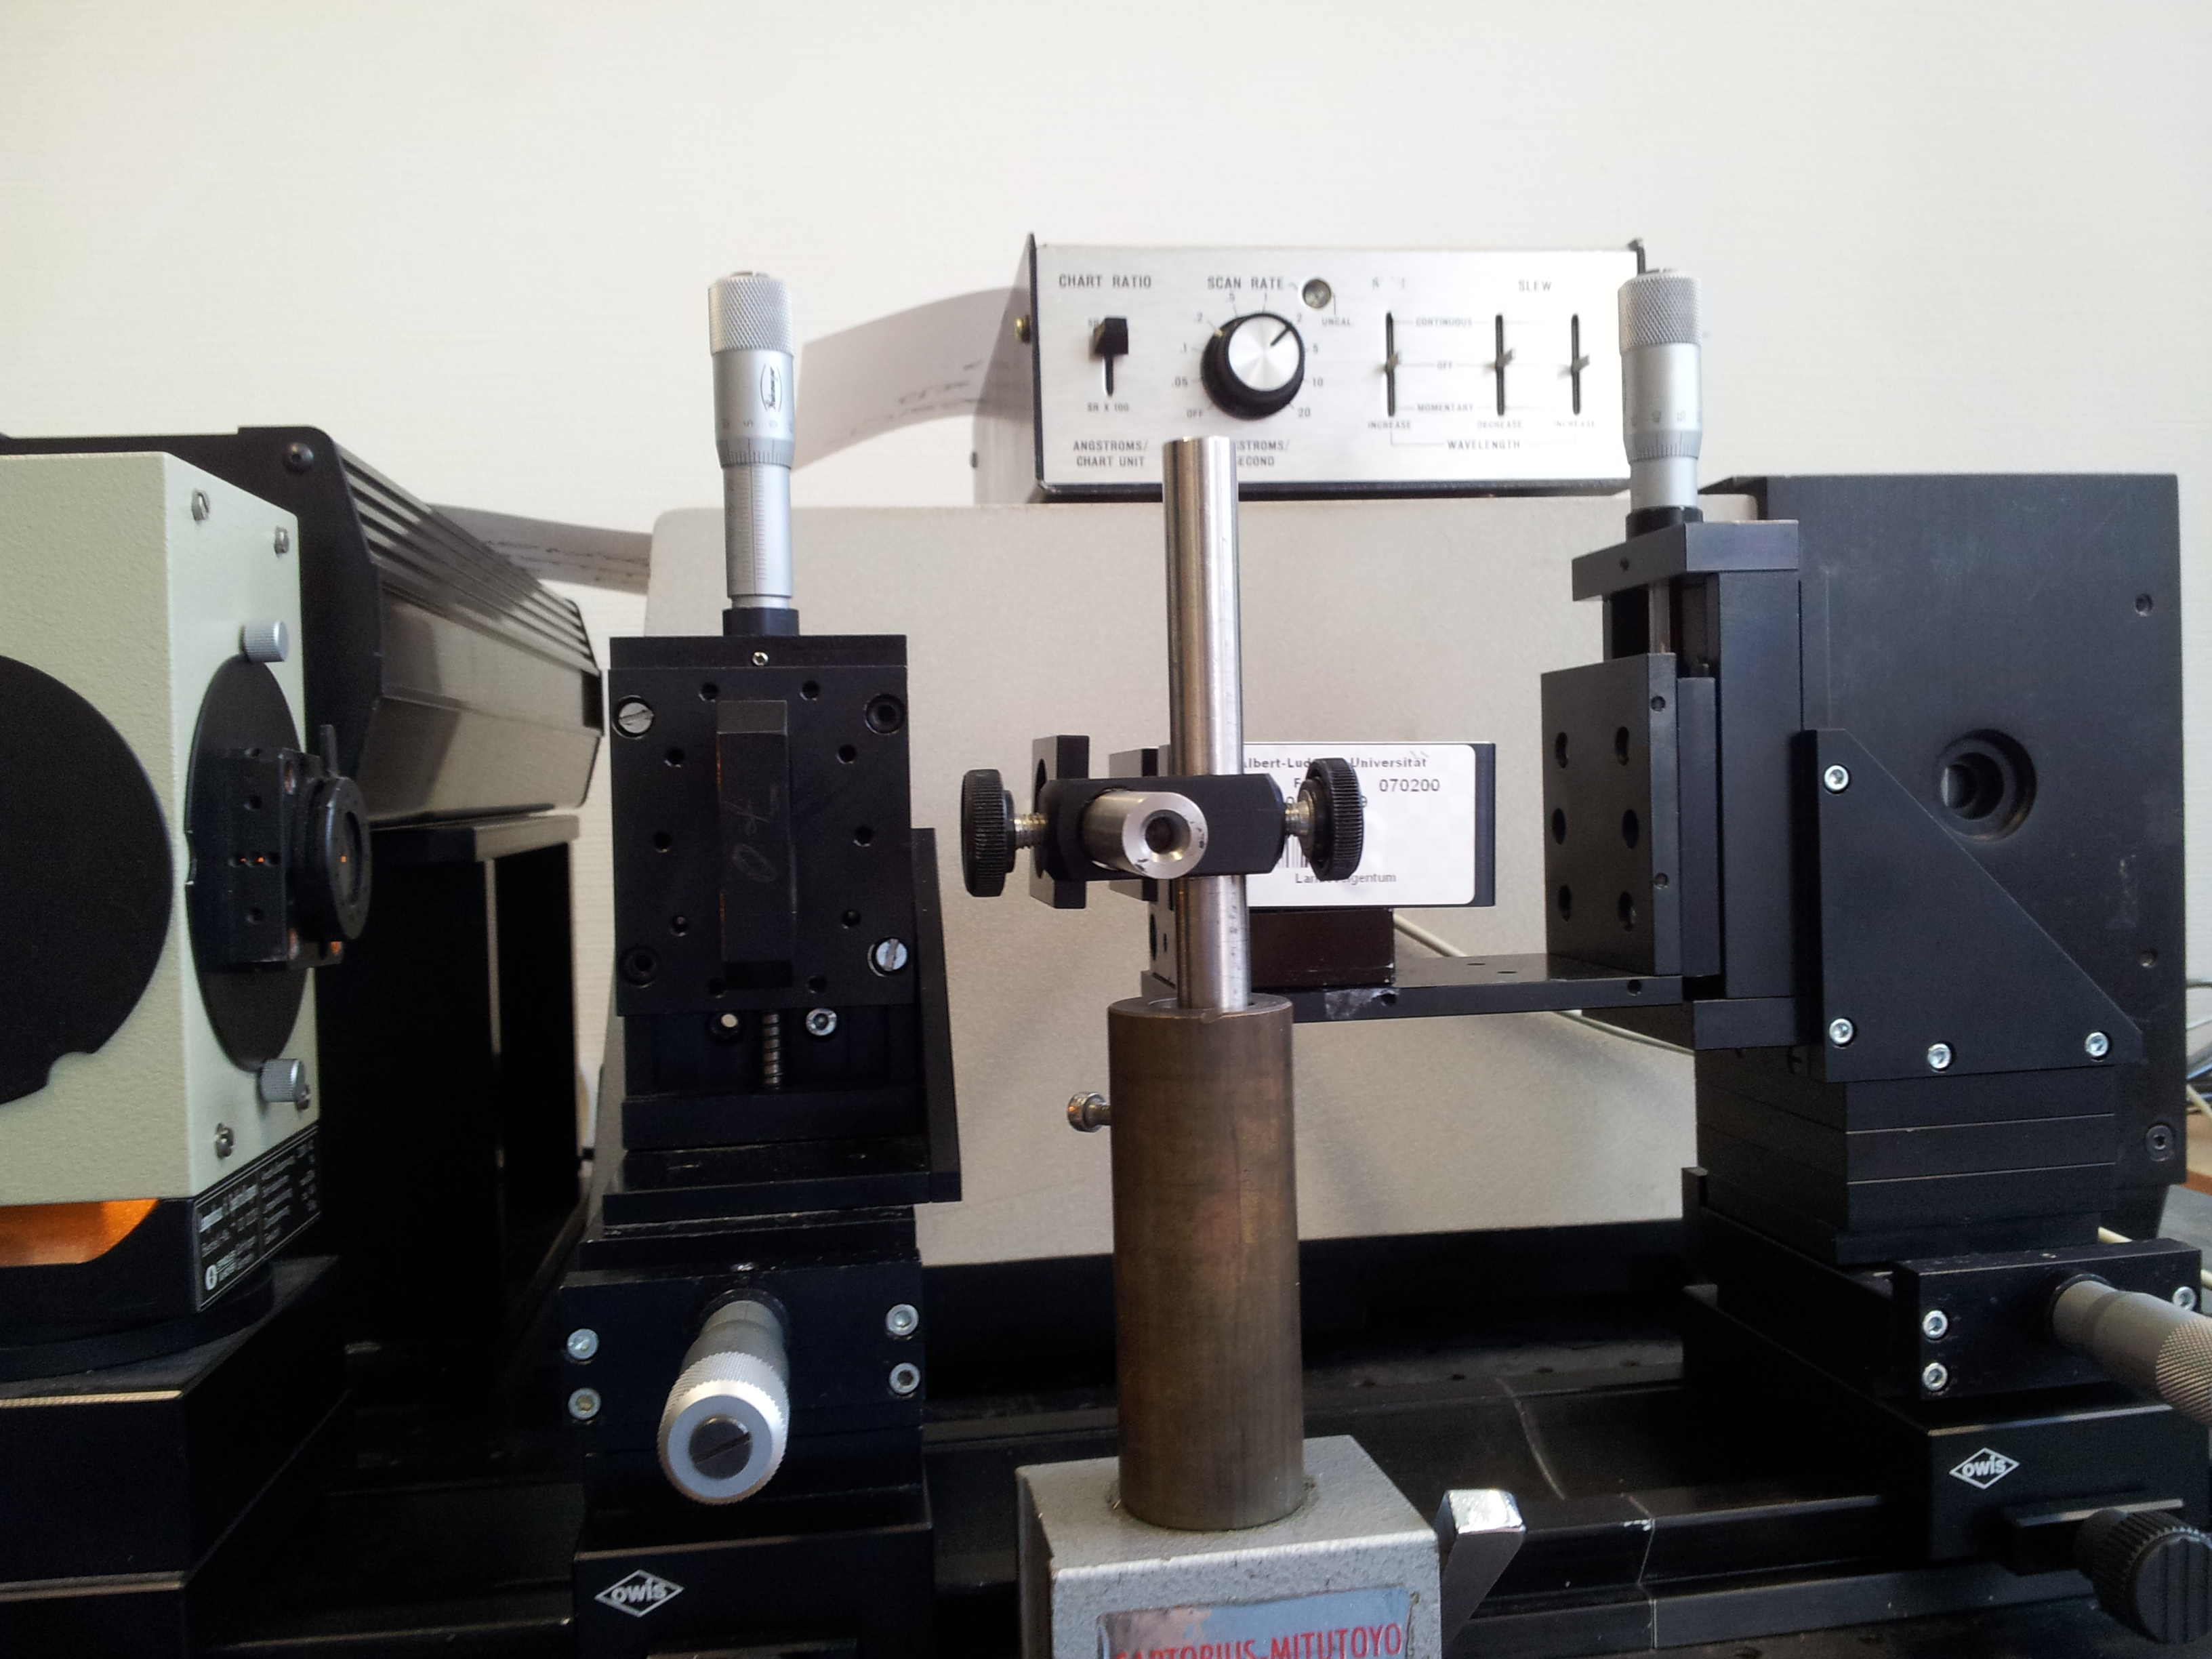
\includegraphics[width=0.48\textwidth]{pics/const1}
  \end{center}
\caption{Photography of the experimental setup when we measure
    the spectra of the given lightsources. The little white box is
    the spectroscope.} 
 \label{fig:const1}

\end{wrapfigure}
\subsubsection{CCD-Spectroscope}
The Device itself was invented 1969 at the 
\textit{AT\&T Bell Labs}. It is a Charge Couple Device (CCD) and it uses
the photoeffect for translating the information of the wavelength
of the photon into a potential difference, which can be saved
in terms of condensators. So effectively the number of electrons
resample the number of incoming photons.
It consists of a high-sensitivity 2048-element CCD array 
(see table~\ref{tab:ccd} for more details) and each of this
CCD-Sensor is roughly a photodiode, meaning a doped
semiconductor with isolaters which in combination is triggered
by photons: If the energy of the photon is higher than the 
bandgap of the semiconductor, electrons will be lifted from the
valenceband to the conductionband and current-anticurrent pairs
will lead the conducters to save this information. In our case
the incoming light is splitted into its spectral components with
a lattice, these single components are then measured by the 
CCD-Cells such that we measure the given Spectral window 
we are to look at. We use the \textit{USB2000+} of the company \textit{ocean optics}
\cite{versuchsanleitung}. 
The opening is 20 $\mu m$ and the wavelengths which will be
detected are 421 to 617 nm with a spectral resolution of 0.6 nm.
After detecting 
the photons they will be visualized at the computer, where we
can save the given spectrum to a file within the given software
\textit{SpectraSuite}. There are two possibilites to adjust
the received data from the spectroscope:
\begin{itemize}
    \item Integrationtime: This manipulates the timespan in 
        which the incoming photons will be counted. Obviously
        this also regulates the relative Intensity of the signal
        visible in the program, either
        if the required signal was too intense or weak.
    \item Meanvalue over a number of signals: We can adjust
        whether we want to average the incoming signal due to
        a flickering or noise and over how many incoming signals
        should be averaged.
\end{itemize}

\begin{SCfigure}
    \caption{Setup with iodinepipe, where the light of the
        halogenlamp will be transmitted through. On the right side
        you can recognize the spectroscope, which will measure
        the absorption lines of the iodine-2 molecules, which
        are located inside of this pipe. It is necessary
        to evacuate them inside of the pipe, because otherwise it
        would sublime in the air.
        } 
    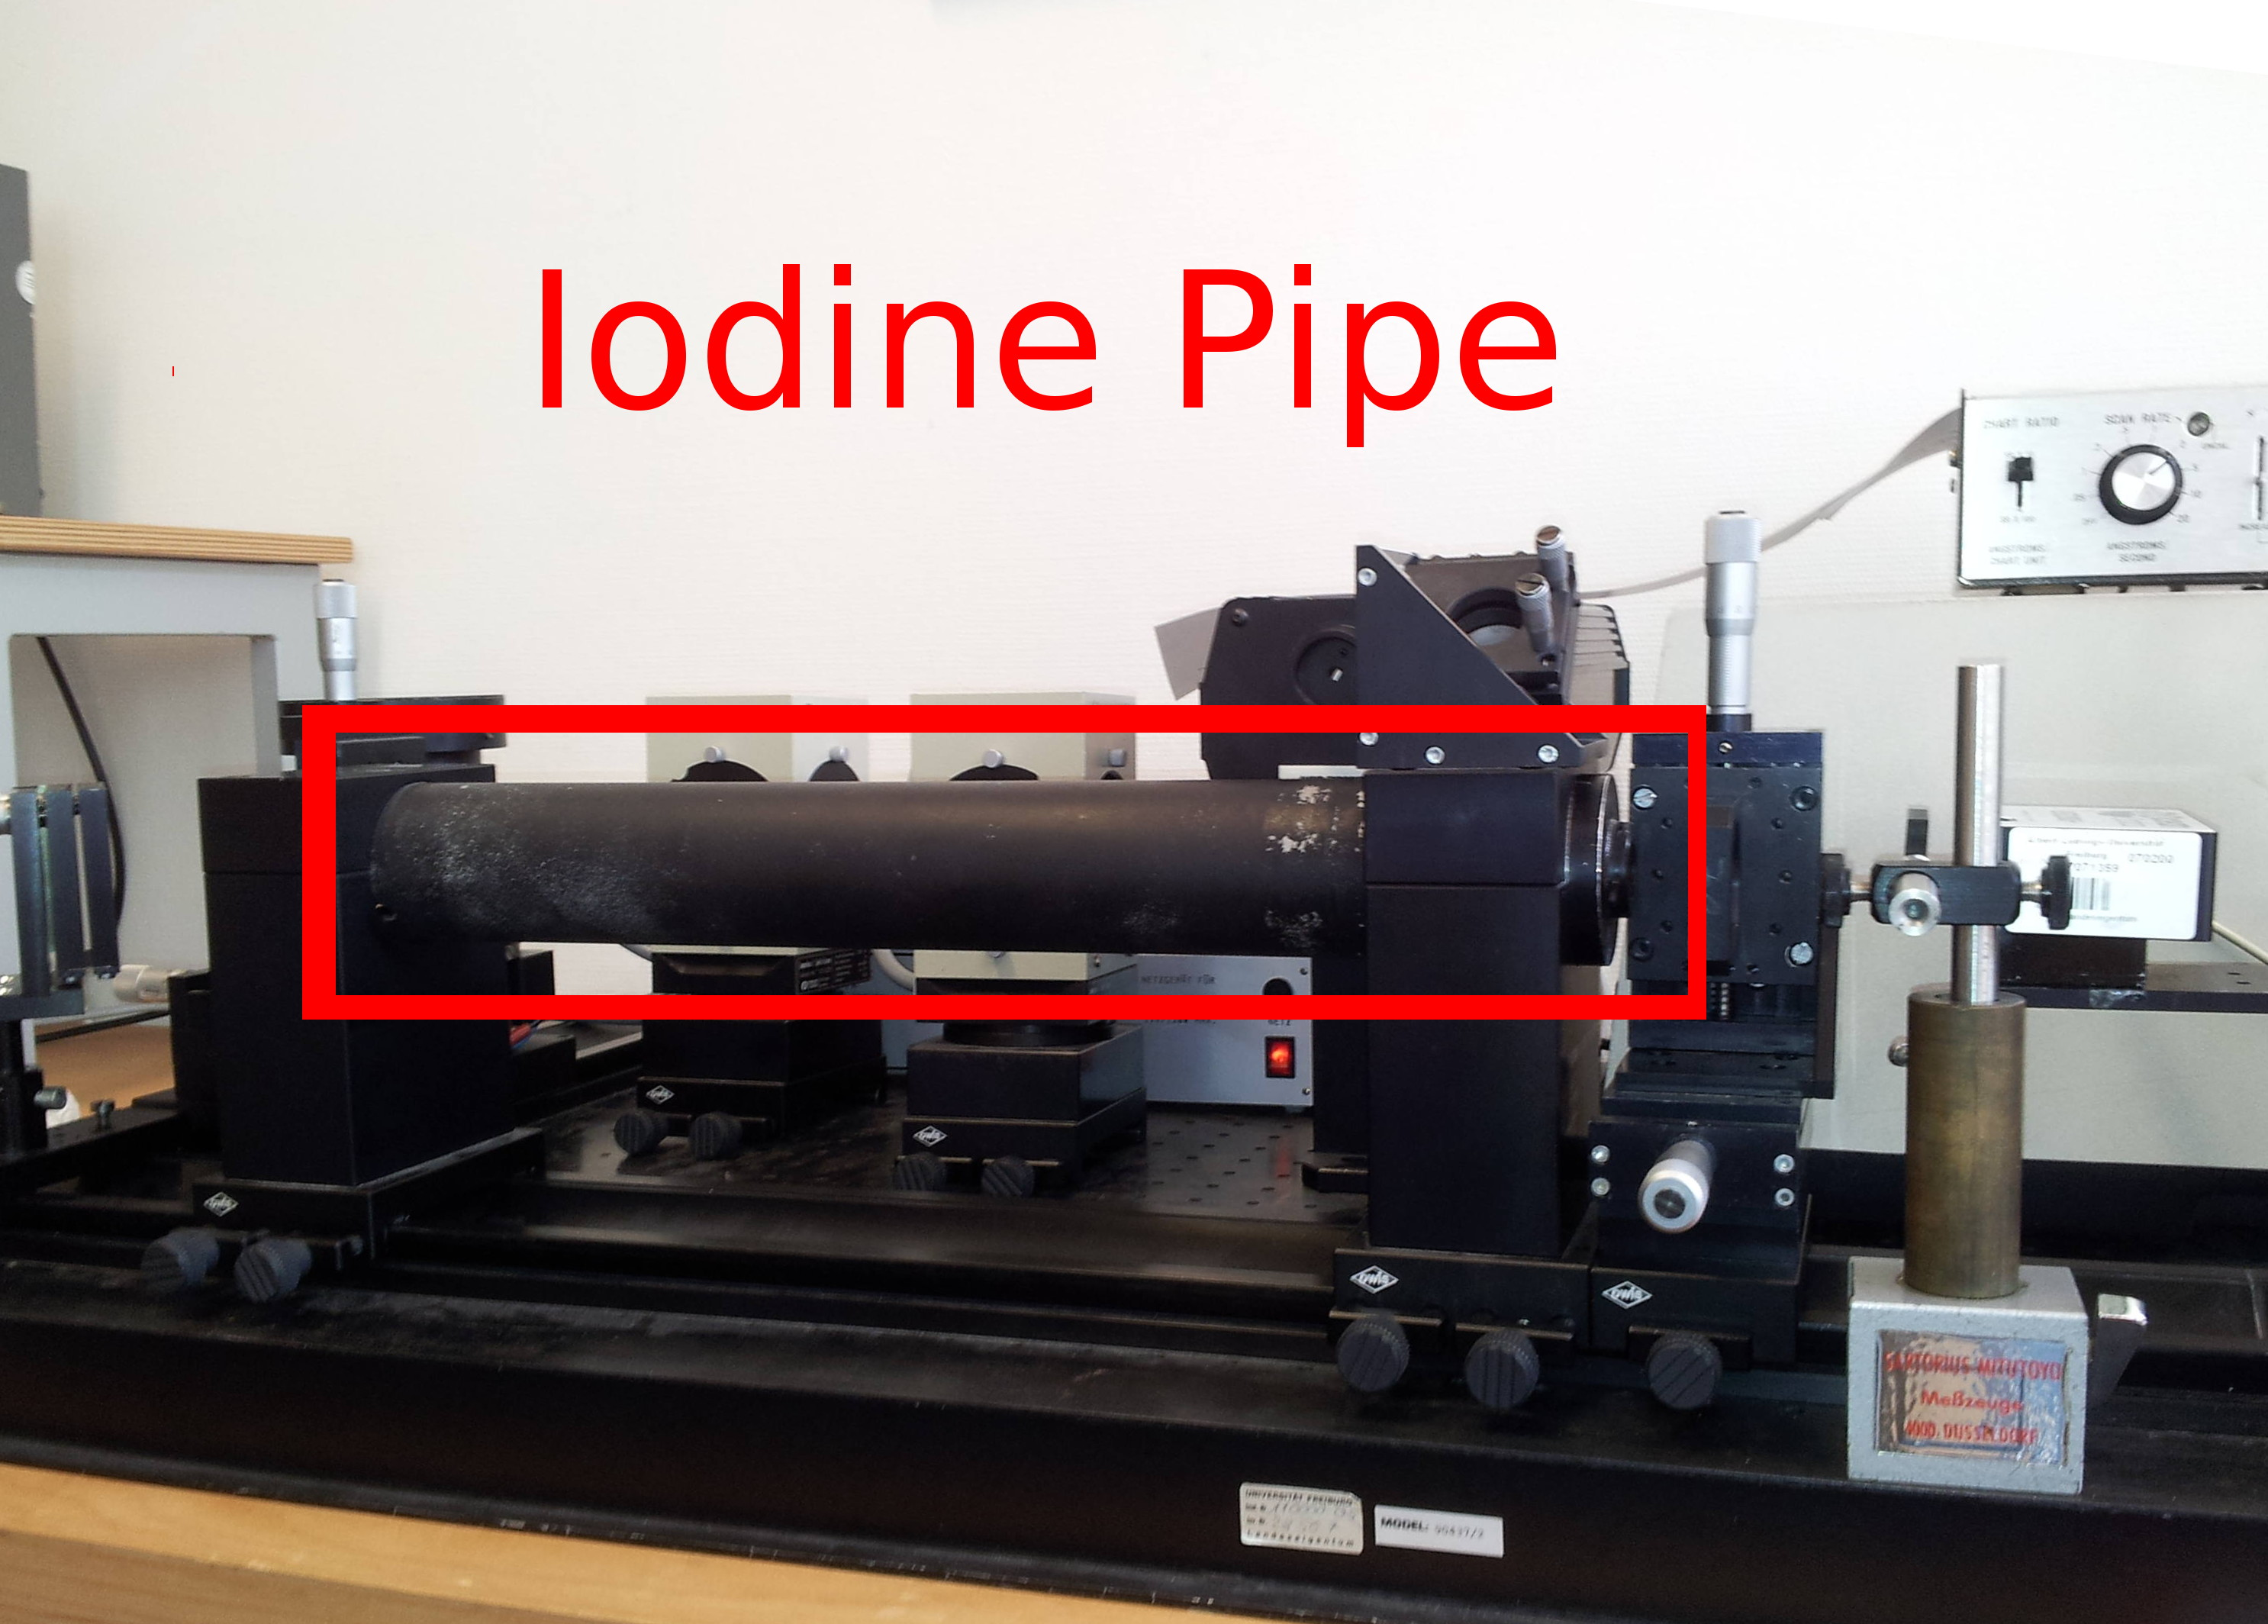
\includegraphics[width=0.48\textwidth]{pics/const2}
 \label{fig:const2}
\end{SCfigure}

\begin{wraptable}{h}{7cm}
    \caption{Specifications of the  CCD Camera \textit{usb2000+}
        \cite{usb2000_site}.}
\begin{tabular}{| l | l |}
    \hline
    Dimensions & 89.1 mm x 63.3 mm x 34.4 mm \\ 
    \hline
    Detector & Sony ILX511B (2048-element \\
             & linear silicon CCD array) \\  
    \hline
    Range & 200-1100 nm \\ 
    \hline
    Pixels: & 2048 pixels \\ 
    \hline
    Pixelsize & 14 µm x 200 µm \\ 
    \hline
    Optical resolution: & 0.3-10.0 nm \\ 
    \hline
\end{tabular}
\label{tab:ccd}
\end{wraptable}

\subsubsection{Spectra of light sources}
In this experiment we will use the nearly continuos spectrum of
the halogenlamp, but before we will calibrate the spectroscope
with the spectra of the other lamps as following.
Since we have very precise values for the emissionspectra of 
the given lightsources \cite{nist} we now immedeatly if
there is a shift in wavelengths (These values for will be given
in the evualation of our results when we compare them with our
results).

\begin{SCfigure}
\caption{Photography of the experiment including the mirrors on
    the left side, the lenses and the opening of the iodinepipe.
    Behind of the lenses there is the lamp whose spectrum will
    be analyzed in the spectroscope, after being transmitted
    through the iodinepipe.} 
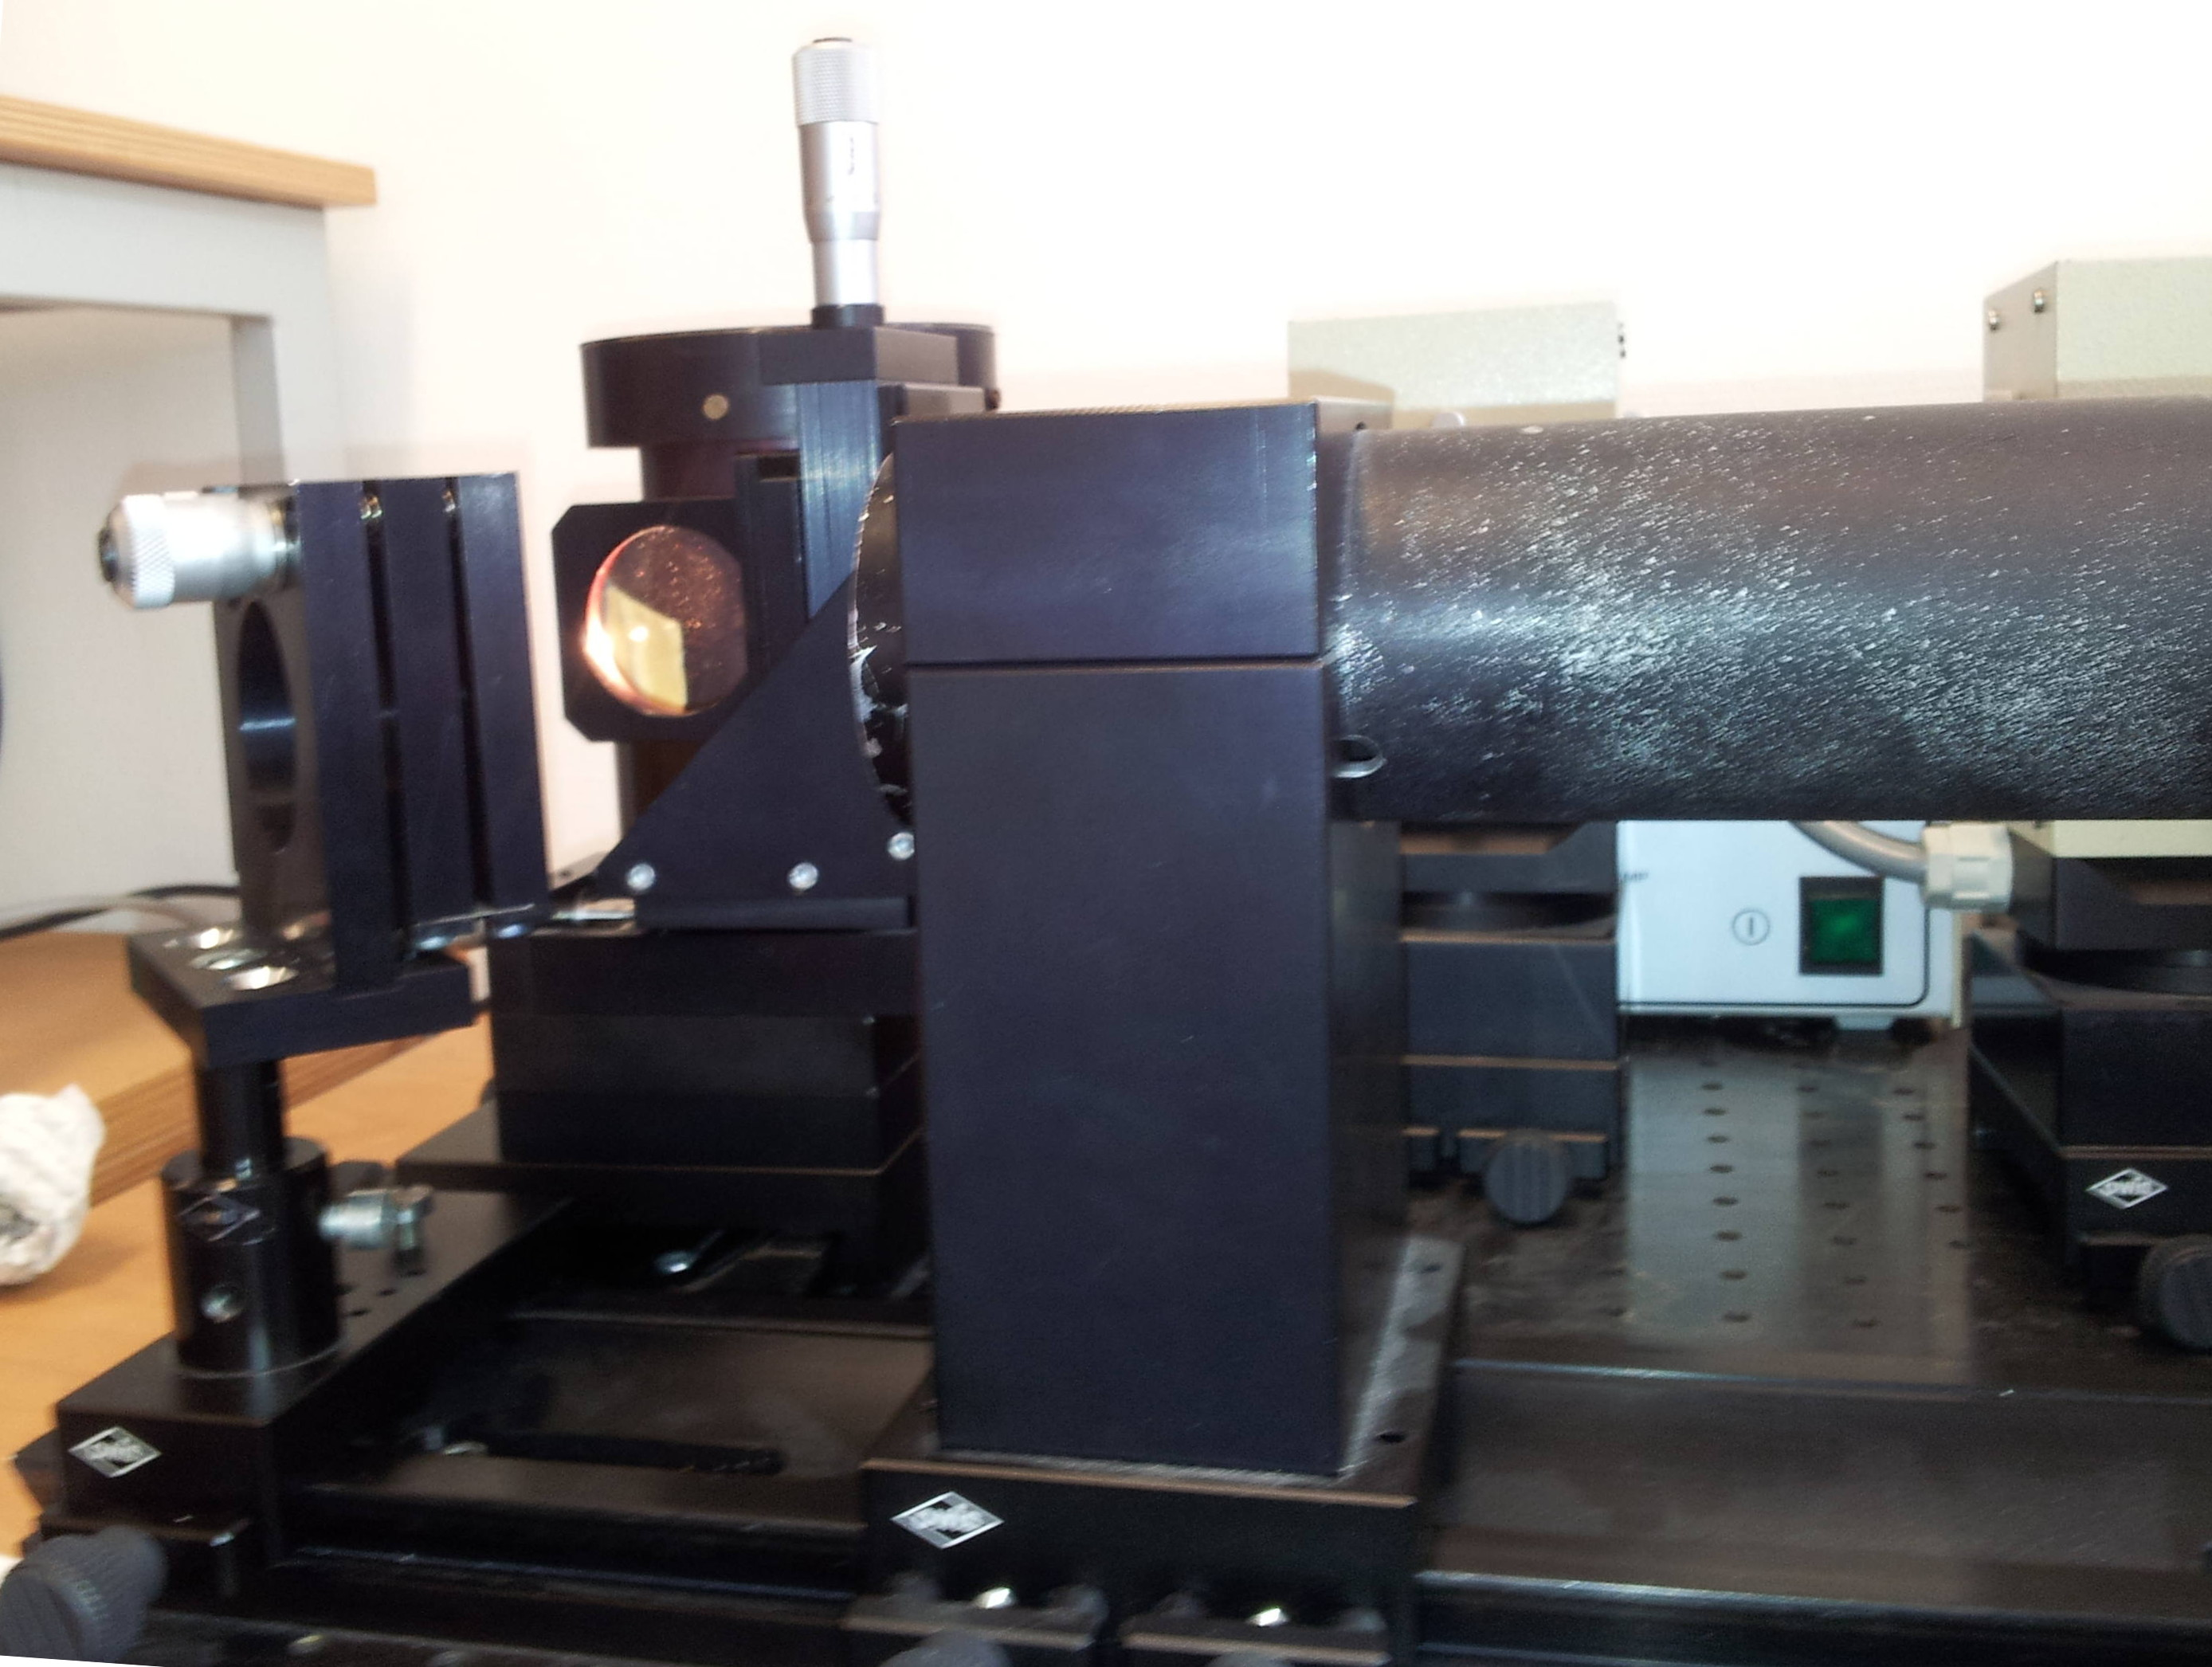
\includegraphics[width=0.47\textwidth]{pics/const4}
 \label{fig:const4}

\end{SCfigure}

\begin{SCfigure} 
\caption{This picture shows the perpendicular view of the
    experimental setup, in which you can recognize clearly
    the CCD-Spectroscope (the white box). } 
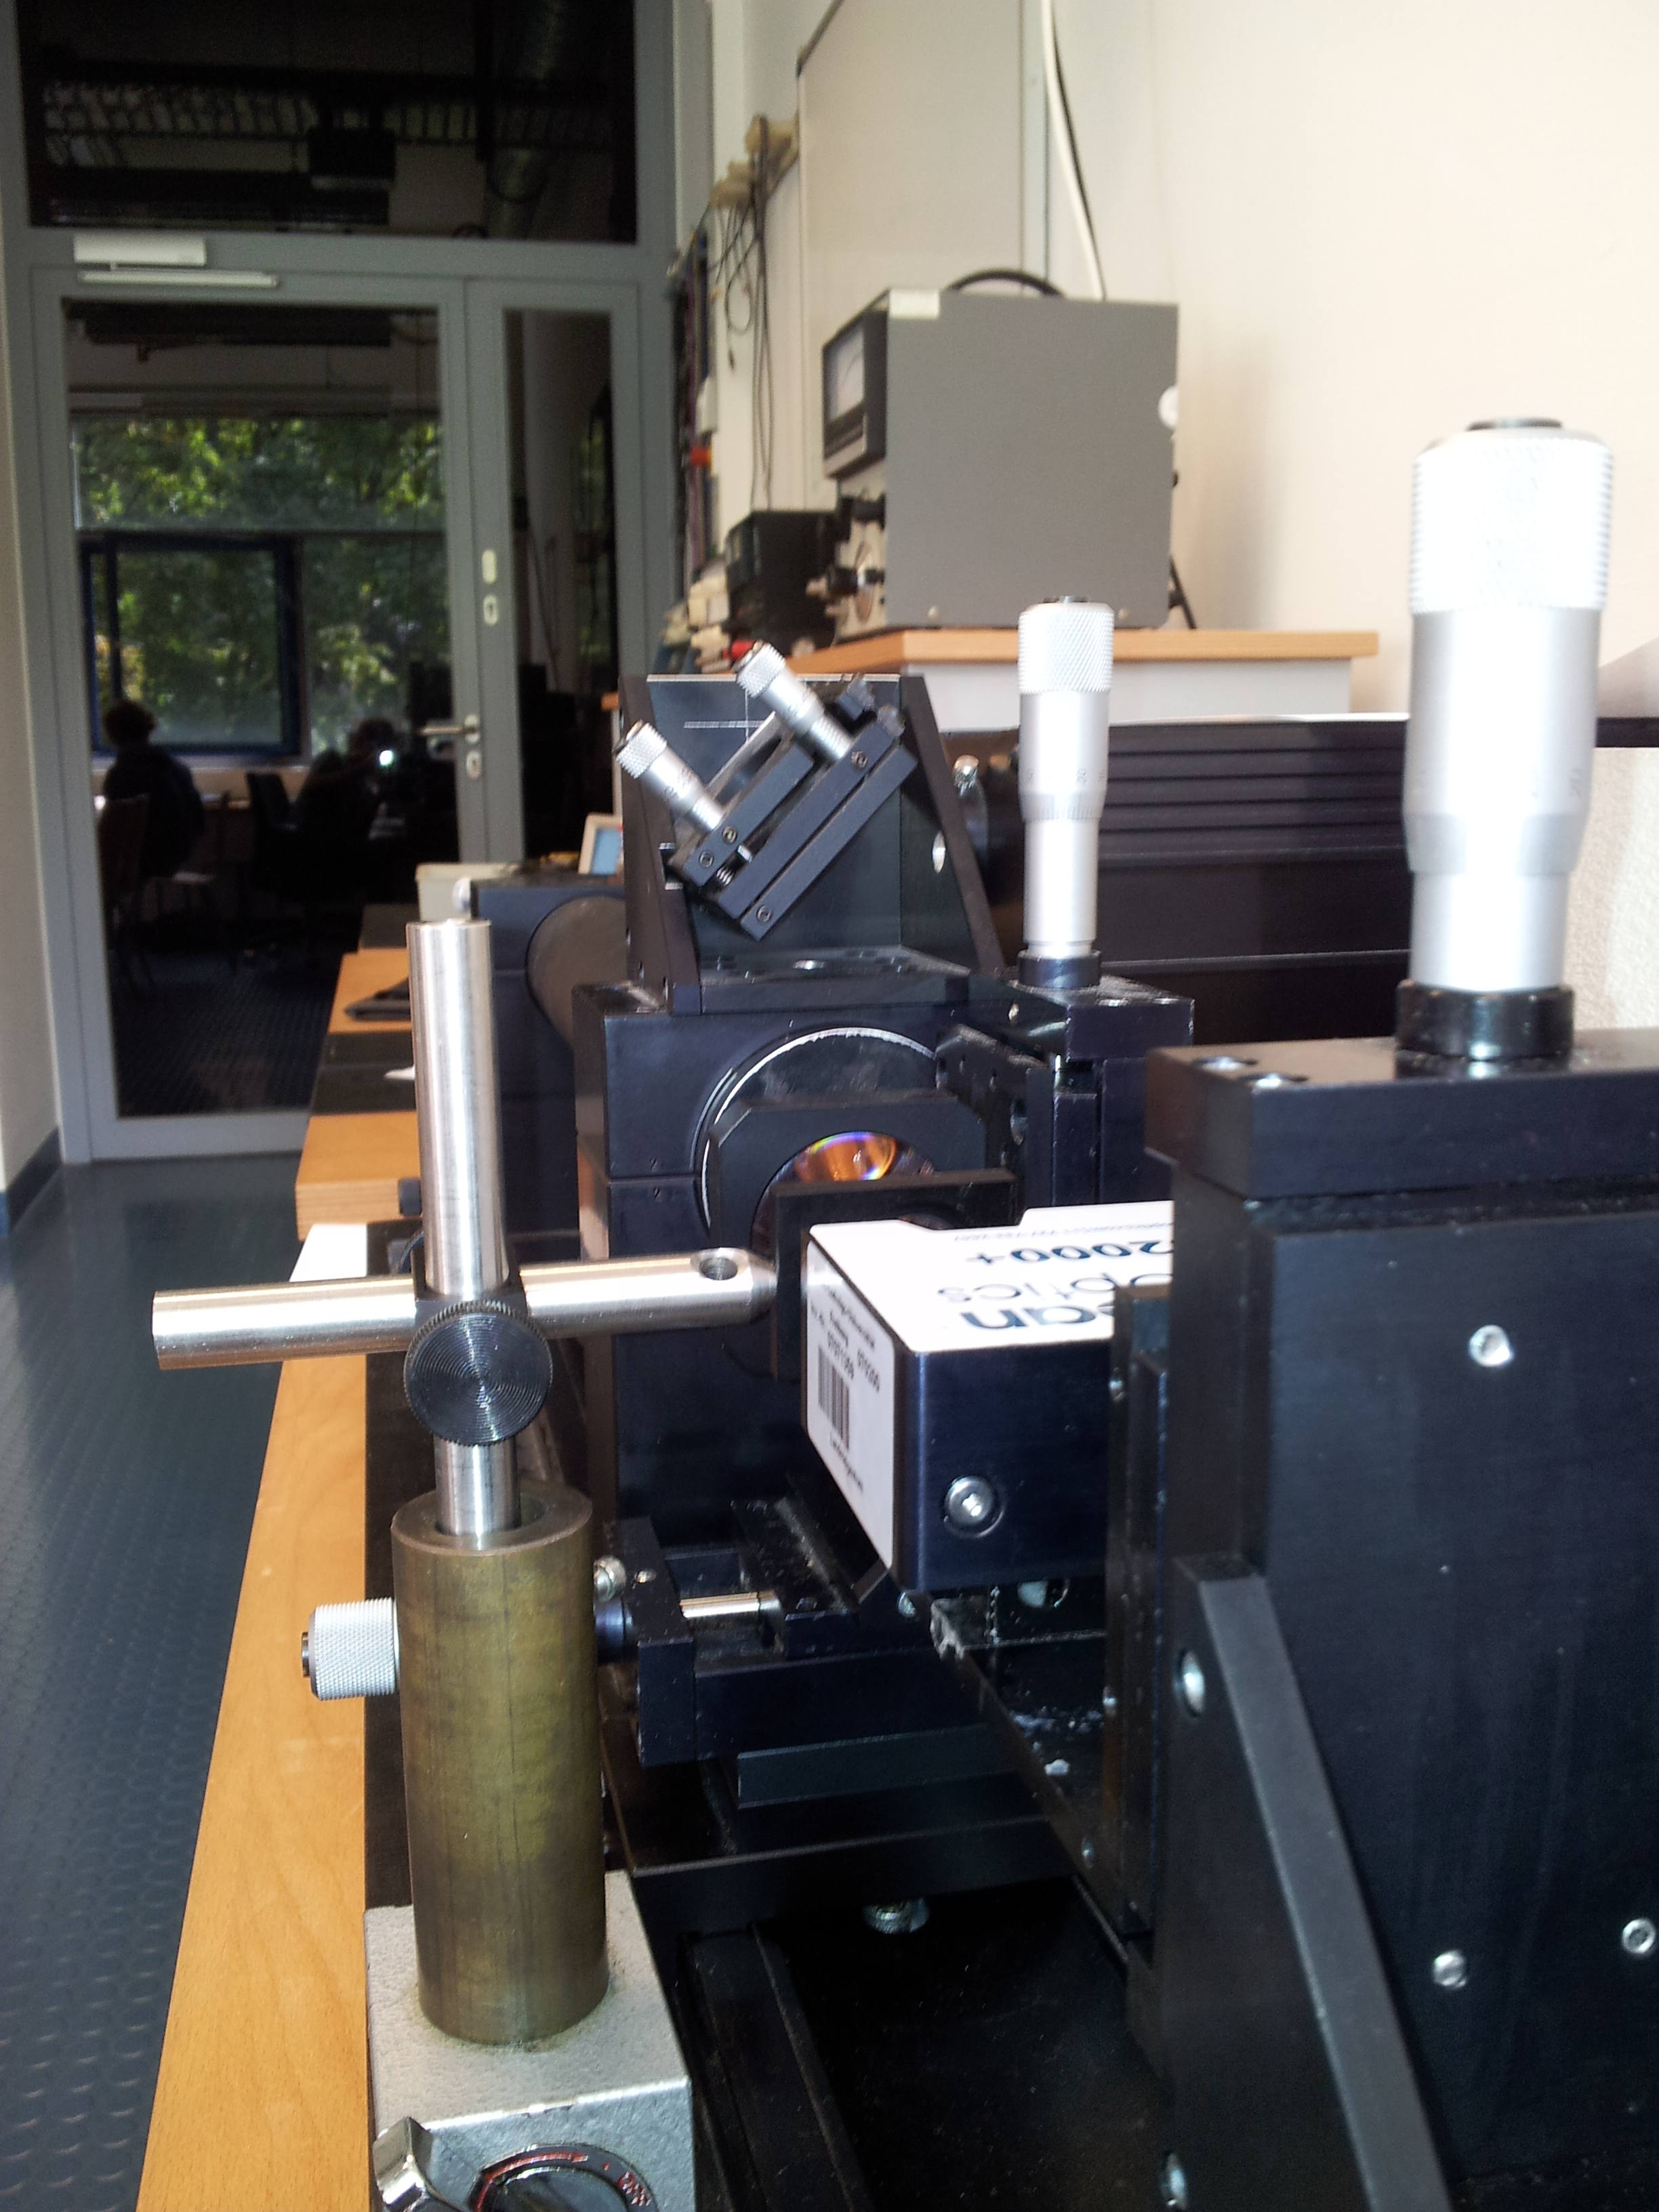
\includegraphics[width=6cm]{pics/const3}
 \label{fig:const3}
\end{SCfigure}

